%=================================================================
\documentclass[dvipdfmx]{issj}
%=================================================================
% 情報システム学会 研究発表大会 原稿用テンプレートの利用例
%     ISSJ実行委員会/プログラム委員会(ISSJ学会誌編集委員会)
% issj2012.sty Ver. 0.50 2012-10-12 Tadashi Iijima (iijima@ae.keio.ac.jp)
% issj2012.sty Ver. 0.60 2012-10-15 Tadashi Iijima (iijima@ae.keio.ac.jp)
% issj2012.sty Ver. 0.70 2012-10-19 Tadashi Iijima (iijima@ae.keio.ac.jp)
% issj2012.sty Ver. 0.80 2012-10-20 Tadashi Iijima (iijima@ae.keio.ac.jp)
%=================================================================
\title{「Twitter上で共感を生み出すツイートの性質に関する考察」の検証}
%-----------------------------------------------------------------
\etitle{Verification of "Consideration on Characteristics of Sympathy-arousing Tweets on Twitter"}
%-----------------------------------------------------------------
\author{木村 咲\uddag, 松澤芳昭\uddag}
%-----------------------------------------------------------------
\eauthor{Saki Kimura\udag, and Yoshiki Matsuzawa\uddag}
%-----------------------------------------------------------------
\affiliation{\dag 青山学院大学 社会情報情報学部\ddag }
%-----------------------------------------------------------------
\eaffiliation{\dag School of Social Informatics, Aoyama Gakuin University.}
%-----------------------------------------------------------------
%=================================================================
\begin{document}
%=================================================================
\maketitle
%=================================================================
\begin{abstract}
本研究では、先行研究で実証されていた「Twitter上で共感を生み出すツイートの性質」の再現性を確認するための追試を行った。 追試では先行研究とは異なるツイートデータを対象とし、新たに属性として「画像の有無」と「感情極性値」を追加した。 芸能人4名のデータを収集して分析した結果、全ての属性においてTwitterで共感を生み出す性質は見られなかった。 これは先行研究と(A)ツイートの時期、(B)ラベル付けした被験者が異なるためだと考えられる。
\end{abstract}
%=================================================================
\section{はじめに} %%%% 第1節
%=================================================================

近年はSNS上で買い物ができたり、またYoutuberやインスタグラマーなどSNSを使った職業も増え、今後よりSNSマーケティングは盛んになると考えられる。
中でもSNSを運用するにあたって共感の注目が高まっており、日本企業の約63.9%が「SNS運用でユーザーの共感の獲得が目標の指標になっている」と答えている[1]
SNSで注目されている共感だが、共感については動物行動学、教育心理学、社会心理学、臨床心理学や脳神経生理学など他分野で多面的、学際的にアプローチされ、研究が行われており、その時々で共感の定義そのものも、多様であり、捉え方も様々である。[2]

そこで本稿では、Twitterで共感を生み出すツイートはどのような性質があるのかを調査する。





%========================================================================
\section{先行研究と本研究の目的}  %%%% 第2節
%========================================================================

共感は、従来さまざまな観点から多くの分野で研究されてきた。

Twitterにおいての共感の研究では、大川, 高間[3]が、不特定の相手向けになされたツイート(つぶやき)に対し多数の人が共感を抱くケースに着目し、その発生のメカニズムの解明を行っている。
不特定多数のユーザーが閲覧するツイートを対象とするため著名人のツイートデータを対象とし、第一著者の判断により共感が発生しているか否かのラベル付けを行うと同時に、それらのツイートの「fav(いいね数)」や「rt(RT数)」「characters(文字数)」など計11個の属性(表1)の値を取得した。
その結果、「文字数が少ないツイート」と「悲しみを含むツイート」が共感を生み出しやすいことが判明した。文字数が影響を及ぼしてる理由としては、ツイートの長さが冗長であればあるほどユーザーがテキストの全てを閲覧することがなくなり、共感の発生を妨げる原因になってる可能性があるからだ。また、悲しみを含むツイートが影響を及ぼしている理由としては、悲しい記憶は人間の心に残りやすく、そのためツイートを投稿したユーザーの状況をイメージしやすくなり、共感が発生する可能性が高くなるためだと考察している。

そこで本稿では、先行研究の結果は異なるツイートデータでも再現可能なのかを検証するため、ツイートのデータ変えて追試を行う。
加えて、ツイートに画像が貼られているとユーザーはツイートの背景をイメージしやすくなり、共感発生の手助けになると考え、新たな属性としてimage(画像の有無)も加え実験を行う。



\begin{table}[h]\centering
\caption{属性名と属性値の形式}\label{tbl:font}
\begin{small}
\begin{tabular}{|c|c|} \hline
属性名            & 属性値の形式\\\hline\hline
fav & real 型, 0~\\\hline
rt  &  real 型, 0~\\\hline
term  & real 型, 0~\\\hline
characters         & real 型, 0~\\\hline
unofficial      &  real 型, 1~140\\\hline
gladness & {yes, no}\\\hline
anger & {yes, no}\\\hline
sadness & {yes, no}\\\hline
pleasure & {yes, no}\\\hline
sadness & {yes, no}\\\hline
agreement & {agree, disagree, neutral}\\\hline
thinking & {positive, negative, neutral}\\\hline
\end{tabular}
\end{small}
\end{table}

\newpage

%========================================================================
\section{共感の定義}  %%%% 第3節
%========================================================================
本稿では先行研究とは異なる共感の定義づけを行う。
先行研究ではTwitterにおける共感を「そのツイートを不特定多数のユー ザが閲覧したときに,投稿した背景が想像でき,そ れに同感できる」ことと定義している。
この定義の場合、ツイートに同感できなければ共感は成り立たないことを意味している。


しかし、佐伯は「同感」と「共感」を別物と捉えている。
佐伯曰く、「同感というのはその人の感じていることと自分の感じていることを同じなのだと思うこと」であり,そこには未知なる世界への探求も、新しい発見もなく、「相手は自分と同じだという確認」があるに過ぎない。
一方の共感は、「白分にはすてきとは思えないが,その良さをわかりたい」というように、「その人が良いといっているのはどういうところなのだろうということを探求して「理解」しようとする。そこにいたる経緯やそこでの状況をしっかり把握して、その場に我が身をおいて、なんとかして、そこでの「良さ」を、心底「納得」しようとする」ことと捉えられている。[4]


また、ロジャーズは共感を「自分が自分が他者であるかのような、しかし”かのようにas if”という状態を失わずに関係する。正確さや感情的要素、意味を持って他者の内部関連気分を知覚すること」と唱えている。


本稿では、この2つをもとに共感を、「不特定多数のユーザーがそのツイートを閲覧したとき、投稿した背景が想像でき、そのツイート(投稿者)の内部関連気分を汲み取れること」と定義する。
ゆえに共感のラベル付けは、以下の2つの条件が成り立つときに行う。

\begin{table}[h]\centering
\caption{ラベル付けの判断基準}\label{tbl:font}
\begin{small}
\begin{tabular}{|c|c|} \hline
No   & 条件内容\\\hline\hline
条件1& ツイートの背景が記載されているツイート\\\hline
条件2 & 投稿者の感情が汲み取れるツイート\\\hline
\end{tabular}
\end{small}
\end{table}


%------------------------------------------------------------------------
\subsection{ツイートの収集と共感のラベル付け }  %%%% 第3.1節
%------------------------------------------------------------------------
今回は芸能人の中でもフォロワー数が最も多い芸能人男女4名を分析対象とし、2021年7月27日から最新のツイートをそれぞれ50件収集した。
このとき、第一次情報源でない「公式リツイート」と、特定の相手を対象としたつぶやきである「リプライ」は除いている。
TwitterAPIを用いてツイートを取得したツイートに対して共感したか否かを手作業によってラベル付けを行った。


ラベル付けの例を表3に示す。
左は「共感を生み出す」とラベル付けされたツイートである。
このツイートからは、吉高由里子が”自分の誕生日に周りに祝ってもらって嬉しくてツイートした”という背景(条件1)と、”祝ってもらって嬉しい”という感情(条件2)が読み取れる。
一方で、右は「共感を生み出さない」とラベル付けされたツイートである。
このツイートからは、吉高由里子が”誰かと手持ち花火をしている”というツイートの背景が確認できる(条件1)。
しかし、感情面については言及されていないため判断することができない。
つまり、条件2を満たしていないため共感を生み出さないツイートとラベル付けした。

\begin{table}[h]\centering
  \caption{共感を生み出すツイートの例}
  \begin{tabular}{|c|c|} % l:左寄せ,c:中央揃え r:右寄せ 
    \hline \rm 共感を生み出すツイート & \rm 共感を生み出さないツイート \\ \hline
    \hline
    \begin{minipage}{70mm}
      \centering
      \scalebox{0.3}{
\includegraphics{fig1.png}}
    \end{minipage} &
    \begin{minipage}{70mm}
      \centering
      \scalebox{0.3}{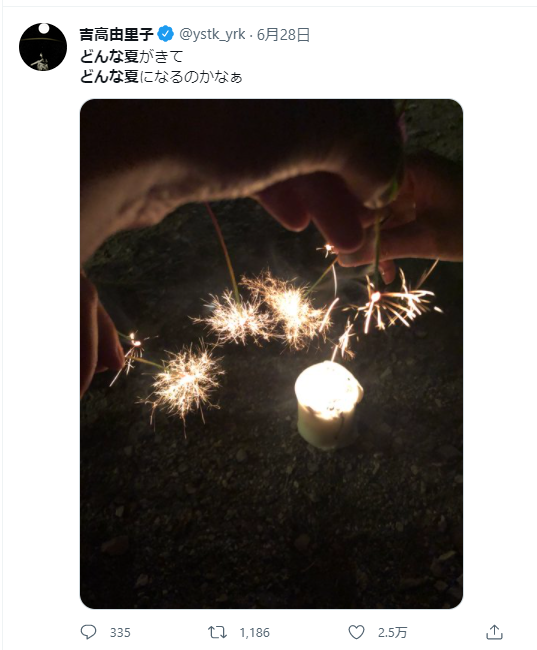
\includegraphics{fig2.png}}
    \end{minipage} \\ \hline
  \end{tabular}
  \label{pic} % \ref{ラベル名}で表番号を参照
\end{table}



%------------------------------------------------------------------------
\subsection{属性の定義と抽出方法}  %%%% 第3.2節
%------------------------------------------------------------------------
ここでは本稿で用いる属性について説明する。本稿で用いる属性を表4に示す。
先行研究で共感の発生と関係があるとされていた「文字数」と「悲しみの感情」は本当に共感発生に影響を及ぼしているのか、そして「画像の有無」も共感発生の手助けになってるのではないかを検証するため、以下の3つの属性を用いる。

1つ目のcharacterは対象ツイートの文字数を指している。先行研究ではツイートの長さが冗長であればあるほど共感の発生を妨げる要因になってるのではないかと考えられていた。[3]
2つ目のimageはツイートに画像が添付されているか否かを表している。画像の有無は読み手にツイートした背景を容易にイメージしやすくさせる役割を果たし、共感発生にも影響を及ぼしているという仮説をもとに新たに属性として加えた。
最後にemotion valueはツイートテキストのネガティブ(ポジティブ)評価ができる感情極性値を指している。先行研究では感情語辞書を作成し、ツイートテキストに喜怒哀が含まれているかどうかを分析を行っていたが、本稿では感情極性値を用いる。この値は最小に近くなるほど、そのツイートはnegativeだと判断できる。

表4に示した各ツイートの属性値を「説明属性」、共感発生の有無を「目的属性」と定めてデータセットを作成し、適合率、再現率により性能を評価する。



%%%% 表:属性名と属性値の形式
\begin{table}[htbp]\centering
\caption{属性名と属性値の形式}\label{tbl:font}
\begin{small}
\begin{tabular}{|c|c|} \hline
属性名            & 属性値の形式\\\hline\hline
characters         & real 型, 0~\\\hline
image & {yes, no}\\\hline
emotion value     &  real 型, -1~1\\\hline
\end{tabular}
\end{small}
\end{table}

\newpage


%========================================================================
\section{結果と考察}  %%%% 第4節
%========================================================================


%------------------------------------------------------------------------
\subsection{結果}  %%%% 第4.1節
%------------------------------------------------------------------------
データセットは前述のフォロワー数が多い男女4名の芸能人のツイートから、2021年7月27日において最新のツイートから時系列順に数えて50件取得した。(表5)

今回設定した3つの属性に対して、適合率、再現率、正解率を算出したデータを以下に示す。性能評価では、先行研究と同様に再現率を重視し、再現率が7/10以上でかつ適合率が1/3以上となるものを選択した。

その結果、どの属性においても上記の条件に当てはまるものが見られず、共感を生み出す性質はどの属性においても確認できなかった。



%%%% 表:データセットの概要
\begin{table}[hbtp]
  \caption{データセットの概要}
  \label{table:data_type}
  \centering
  \begin{tabular}{lcr}
    \hline
   ユーザー名 & フォロワー数  &  共感発生数  \\
    \hline \hline
吉高由里子 & 310.0万人 &  22/50  \\
ベッキー & 195.1万人 &  25/50  \\
松本人志 & 818.9万人 &  20/50  \\
有吉弘行 & 671万人 &  6/50 \\
    \hline
  \end{tabular}
\end{table}




%------------------------------------------------------------------------
\subsection{考察}  %%%% 第4.2節
%------------------------------------------------------------------------
1つ目のcharacters(文字数)は、先行研究とは異なる結果が得られた。
先行研究では、文字数がある値以下のときに共感を生み出す判定する学習う結果が多く見られ、ツイートの文字数が多く冗長であればあるほど、ユーザーがテキスト全てを閲覧することがなくなってしまい共感発生を妨げる要因になってるのではないか、また要点がまとまっている短めの文章の方が共感を発生させやすいのではないかと考察していた。

しかし、本稿のデータからは文字数の多さと共感発生に関係は見られなかった。

認知的共感(相手の立場や視点に立って、考え方や感じ方を理解するといった認知的側面が優位な共感)に基づいて考えると、共感するにはまず相手の状況をしっかり理解する必要がある。

そのため、ツイート内容に投稿した背景が含まれているほど、共感は発生しやすくなると考えられる。

つまり、描写や背景などしっかり書かれている文字数が多いツイートの方が共感を得やすいのではないかという仮説を立てることができる。


2つ目のimage(画像の有無)は、投稿した背景や投稿内容がイメージしやすく共感が発生しやすいと予想していたが、これも同様に共感発生との関係は見られなかった。

画像を用いることでツイートの背景や内容を理解しやすくなるという側面はあるが、その画像の内容にもよるのかもしれない。
今後はツイート内容と画像の内容がマッチしているのか、なども踏まえたうえで分析する必要がある。

最後にemotion value(感情極性値)も共感発生との関係は見られなかった。
これはツイートのラベル付けを行う人のに依存するように思える。
例えば、ポジティブな人はポジティブなツイートの方が共感しやすいだろう。
今後はラベル付けを行う人を複数にして実験を再度行っていきたい。

%------------------------------------------------------------------------
%------------------------------------------------------------------------
%------------------------------------------------------------------------
%%%% 表:画像
\begin{table}[htb]
  \begin{center}
    \caption{Imageの評価値}
    \begin{tabular}{c|ccc} \hline \hline
& 適合率 & 再現率 & 正解率 \\ \hline \hline
吉高由里子 &0.38&0.27&0.48 \\ \hline
ベッキー &0.5&0.08&0.5\\ \hline
松本人志 &0.67&0.1&0.62 \\ \hline
有吉弘行 & 0.08&0.33&0.46 \\ \hline
    \end{tabular}
    \label{tab:tripcode_user}
  \end{center}
\end{table}


%%%% 表:文字数
\begin{table}[htb]
  \begin{center}
    \caption{Characterの評価値}
    \begin{tabular}{c|ccc} \hline \hline
& 適合率 & 再現率 & 正解率 \\ \hline \hline
吉高由里子 &0.2&0.09&0.44 \\ \hline
ベッキー &0.11&0.16&-0.08\\ \hline
松本人志 &0.32&0.45&0.4\\ \hline
有吉弘行 & 0.09&0.67&0.12 \\ \hline
    \end{tabular}
    \label{tab:tripcode_user}
  \end{center}
\end{table}


%%%% 表:ネガティブ
\begin{table}[htb]
  \begin{center}
    \caption{Negativeの評価値}
    \begin{tabular}{c|ccc} \hline \hline
& 適合率 & 再現率 & 正解率 \\ \hline \hline
吉高由里子 &0.41&0.41&0.48 \\ \hline
ベッキー &0.46&0.44&0.46\\ \hline
松本人志 &0.31&0.45&0.38\\ \hline
有吉弘行 & 0.11&0.33&0.58 \\ \hline
    \end{tabular}
    \label{tab:tripcode_user}
  \end{center}
\end{table}



%========================================================================
\section{おわりに}  %%%% 第5節
%========================================================================

本稿では、先行研究に基づいてTwitterにおいて共感を発生させるツイートにはどのような性質があるのかを調査し考察を行った。

分析結果より、先行研究でいわれていた文字数が少ないツイートが共感を発生させることは検証できなかった。

また、ツイートのポジティブ(ネガティブ)さを表す感情極性値や画像の有無からも共感発生の関係は見ることができなかった。

本稿で用いたデータセットは小規模であるため、今後はより大規模で分析を行う必要がある。また、共感のラベル付けはその人の性格に依存しやすく、人によってラベルの付け方が異なる可能性が高いため、人に依存しないような共感の定義付けを行うことや、複数の評価者による判定でラベル付けを行う必要があると考えている。





%========================================================================
%%%% 参考文献
%========================================================================
\begin{thebibliography}{99}


  \bibitem{bib:SO2014} 坂田利康, 
                       ^^ ^^ SNSマーケティング戦略 Facebookを使った価値共創による商品開発、総合的O2O、ユーザー・アナリティクスの事例による一考察 '' 
                       高千穂論叢 ,Vol.49 No.3, 2014, pp.83-142.
  \bibitem{bib:HV1987}  竹内 淑恵, 
                       ^^ ^^ Facebookページにおける共感の発生要因とコミュニケーション効果 '' 
                       イノベーション・マネジメント ,Vol.13, 2016, pp.126.

  \bibitem{bib:HV1987}  大川 陽聡,高間 康史, 
                       ^^ ^^ Twitter 上で共感を生み出すツイートの性質に関する考察 '' 
                       インタラクティブ 情報アクセスと可視化マイニング研究会 ,Vol.2012 NoAM-02,2012, pp.02-.



  \bibitem{bib:SO2014} 諏訪 正樹,
                       ^^ ^^ 佐伯 胖 (編著) (2017). 『「子どもがケアする世界」をケアする ―保育における「二人称的アプローチ」入門』'' 
                       日本認知科学会 ,Vol.26 No.3, 2014, pp. 389-390.


\end{thebibliography}
%========================================================================
\end{document}
%========================================================================
